% !TeX spellcheck = ru_RU_yo
% !TEX program = xelatex

\documentclass[pta]{../../../../scs-iam}

\begin{document}

\newgeometry{
  top=20mm,
  right=15mm,
  bottom=20mm,
  left=20mm,
  bindingoffset=0cm
}

\thispagestyle{empty}

\begin{center}
  {
    \bfseries
    {
      \subnormal
      Министерство образования и науки Российской Федерации
    } \\[-0.5em]
    {
      \scriptsize
      ФЕДЕРАЛЬНОЕ ГОСУДАРСТВЕННОЕ АВТОНОМНОЕ ОБРАЗОВАТЕЛЬНОЕ УЧРЕЖДЕНИЕ ВЫСШЕГО ОБРАЗОВАНИЯ
    } \\[-0.25em]
    {
      \subnormal
      “САНКТ-ПЕТЕРБУРГСКИЙ НАЦИОНАЛЬНЫЙ ИССЛЕДОВАТЕЛЬСКИЙ \\[-0.5em]
      УНИВЕРСИТЕТ ИНФОРМАЦИОННЫХ ТЕХНОЛОГИЙ, \\[-0.75em]
      МЕХАНИКИ И ОПТИКИ”
    }\\[1em]
  }
  \begin{minipage}{.8\textwidth}
    \titledline{\textbf{Факультет}}
    $\underset{
      \text{\scriptsize (название факультета)}
    }{
      \underline{\makebox[\remaining][c]{программной инженерии и компьютерной техники}}
    }$ \\
    \textbf{Кафедра}
    \hfill
    $\underset{
      \text{\scriptsize (название кафедры)}
    }{
      \underline{\makebox[\remaining][c]{информатики и прикладной математики}}
    }$
  \end{minipage}
\end{center}

\small

\begin{center}
  {
    \normalsize
    \textbf{И Н Д И В И Д У А Л Ь Н О Е\quad З А Д А Н И Е}
  } \\[-0.25em]
  \textbf{на}~$\underset{\text{\scriptsize (название практики)}}{\underline{\makebox[.4\textwidth][s]{\strut\hfill производственную (НИР)\hfill}}}$~\textbf{практику}
\end{center}

{
  \parindent 0pt
  
  \textbf{Студент}
  $\underset{\text{\scriptsize (Фамилия, Имя, Отчество)}}{\underline{\makebox[.65\textwidth][s]{\strut Кузнецов Андрей Андреевич\hfill}}}$
  \hfill
  \textbf{Группа №}
  \underline{\makebox[.1\textwidth][c]{\strut P4215~~}} \\[-1em]
  
  \titledline{\textbf{Руководитель}}
  $\underset{
    \text{\scriptsize (Фамилия И.О., место работы, должность)}
  }{
    \underline{\makebox[\remaining][l]{\strut Фёдоров Е.М., ИП Николаев Д.А., руководитель отдела разработки ПО\hfill}}
  }$ \\[-1em]
  
  \textbf{Тема задания}
  \uline{<<Разработка веб-интерфейса для проведения геодезических изысканий с помощью устройств Emlid Reach и Emlid Reach RS>> \hfill} \\[-1em]
  
  \textbf{Сроки прохождения практики}
  \uline{~05.02.2018 по 29.04.2018 \hfill} \\[-1em]
  
  \textbf{Место прохождения практики}
  \uline{~ИП Николаев Денис Александрович \hfill} \\[-1em]
  
  \textbf{Должность практиканта}
  \uline{~программист \hfill} \\[-1em]
  
  \textbf{1 Виды работ и требования к их выполнению} \\
  \uline{В процессе практики студент должен выполнить ряд работ в соответствии с план-графиком. Все виды работ должны быть выполнены качественно, с обучающей составляющей для практиканта. \hfill} \\
  \uline{При выполнении основной части работ, обучающийся должен пользоваться документацией к ис\-пользуемым устройствам. Отчеты, выполняемые практикантом должны соответствовать регла\-менту и отображать суть выполненной работы. \hfill} \\[-1em]
  
  \textbf{2 Виды отчетных материалов и требования к их оформлению} \\
  \uline{Промежуточные отчётные материалы должны выполняться в срок в свободной форме. Итоговый отчёт о выполненной работе должен быть выполнен в соответствии с регламентом организации. \hfill} \\
  \uline{Отчёт о практике должен соответствовать итоговому отчёту, с сокрытием информации, содержа\-щей коммерческую тайну. Отчёт о практике должен быть выполнен в соответствии с регламентом ВУЗа. \hfill} \\[-1em]
}

\restoregeometry

\clearpage

\newgeometry{
  top=20mm,
  right=20mm,
  bottom=20mm,
  left=15mm,
  bindingoffset=0cm
}

\thispagestyle{empty}

{
  \parindent 0pt
  
  \begin{center}
    \textbf{3 План-график}
    
    \begin{figure}[h!]
      \centering
      \setlength{\fboxsep}{0pt}
      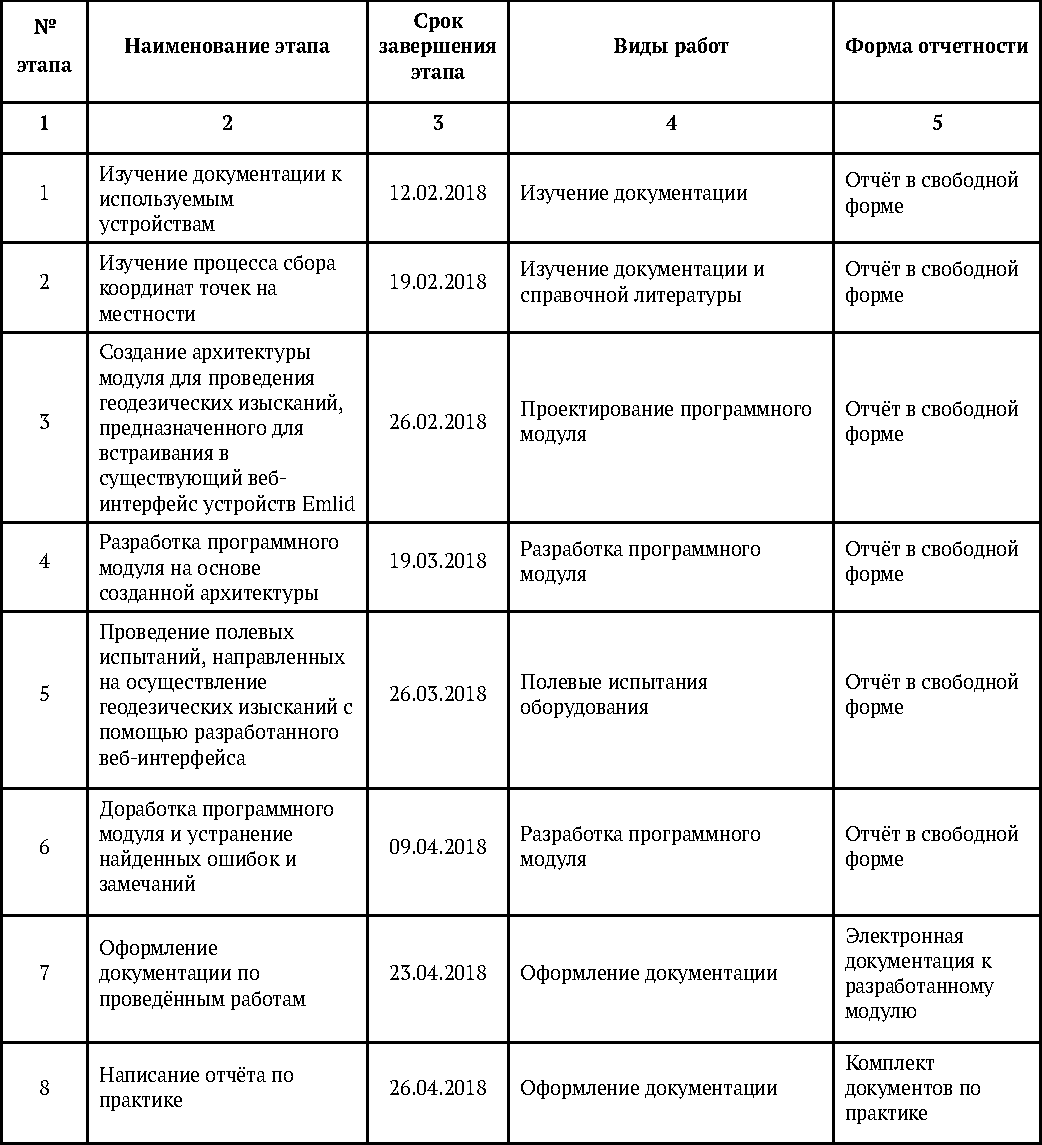
\includegraphics[width=\textwidth]{table}
    \end{figure}
  \end{center}

  {
    \bfseries
    Задание утверждено на заседании кафедры \underline{\makebox[15em][s]{}} \\
    (протокол от \datetemplate~~№\underline{\makebox[3em][s]{}}\,).
  }

  \textbf{Дата выдачи задания}
  \datetemplate
  
  \textbf{Руководитель}
  $\underset{
    \text{\scriptsize (подпись руководителя)}
  }{
    \underline{\makebox[10em][s]{}}
  }$
  
  \textbf{Задание принял к исполнению}
  $\underset{
    \text{\scriptsize (подпись студента)}
  }{
    \underline{\makebox[10em][s]{}}
  }$
}

\end{document}
